%  !TeX  root  =  user_guide.tex

\section{Oracle GeoRaster}

% when the revision of a section has been finalized,
% comment out the following line:
% \updatedisclaimer

В базах данных Oracle, растровые слои могут храниться в объектах
SDO\_GEORASTER, доступных через расширение Oracle Spatial. В QGIS,
\toolbtntwo{oracle_raster}{Модуль Oracle GeoRaster} поддерживается
библиотекой GDAL и зависит от установленной на вашем компьютере базы
данных Oracle. В то время, как Oracle является коммерческим ПО, для
разработки и тестирования оно поставляется бесплатно. Вот один простой
пример того, как загрузить растровые изображения в GeoRaster:

\begin{verbatim}
$ gdal_translate -of georaster input_file.tif geor:scott/tiger@orcl
\end{verbatim}

Эта команда загрузит растр в таблицу GDAL\_IMPORT по умолчанию, в
качестве столбца под названием RASTER.

\subsection{Управление соединениями}

Сначала, модуль Oracle GeoRaster должен быть активирован посредством
<<Управления модулями>> (см. Раздел~\ref{sec:load_core_plugin}). В самый
первый раз, когда модуль GeoRaster загружается в QGIS, требуется
создание соединения с базой данных Oracle, в которой содержатся данные.
Для этого сначала нужно нажать кнопку
\toolbtntwo{oracle_raster}{Выбрать Oracle GeoRaster} на панели
иструментов, откроется диалоговое окно <<Выберите Oracle Spatial GeoRaster>>.
Затем нужно нажать кнопку \button{Создать} для того, чтобы открылось
диалоговое окно и ввести параметры подключения (cм. рисунок~\ref{fig:oracle_create}):

\begin{itemize}[label=--]
\item \textbf{Имя}: ввести название для подключения к базе данных.
\item \textbf{Экземпляр СУБД}: ввести название базы данных, к которой
совершается подключение.
\item \textbf{Пользователь}: ввести имя пользователя, имеющего доступ
к базе данных.
\item \textbf{Пароль}: ввести пароль пользователя.
\end{itemize}

\begin{figure}[ht]
   \centering
   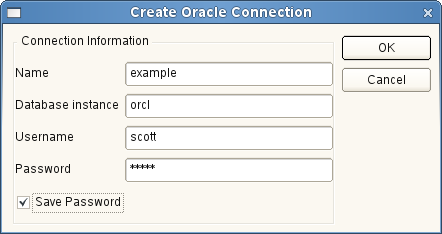
\includegraphics[clip=true, width=9cm]{oracle_create_dialog}
   \caption{Диалоговое окно <<Создать соединение Oracle>> \wincaption}\label{fig:oracle_create}
\end{figure}

Теперь, в диалоговом окне <<Выберите Oracle Spatial GeoRaster>>
(см. Рисунок~\ref{fig:oracle_select}), нужно выбрать подключение из
выпадающего списка и использовать кнопку \button{Подключиться} для
установки соединения. Также существует возможность править параметры
подключения посредством кнопки \button{Правка} или использовать кнопку
\button{Удалить} для удаления соединения из списка.

\subsection{Выбор растровых данных}

После того, как произойдет подключение, в окне блока <<Подчиненные
наборы данных>> появятся названия всех таблиц, содержащих столбцы
растровых данных в формате подчиненных наборов данных GDAL.

Выбрав один из таких наборов данных и нажав кнопку \button{ОК}, можно
выбрать название таблицы. Теперь будет показан другой список подчиненных
наборов данных, содержащий названия колонок растровых данных из этой
таблицы. Обычно это короткий список, так как большинство пользователей
не держит больше 1-2 столбцов в одной таблице.

Выбрав один из приведенных наборов данных и затем нажав \button{ОК},
можно выбрать одну из комбинаций таблица/столбец. Диалоговое окно теперь
покажет все строки, содержащие объекты растровых данных. Заметьте, что
теперь в списке подчиненных наборов данных отображаются пары (таблица
растровых данных:идентификатор растрового изображения).

В любой момент времени можно изменить содержимое строки в блоке
<<Выделение>> для того, чтобы перейти непосредственно к нужному
растровому изображению или вернуться к началу и выбрать другое название
таблицы.

\begin{figure}[ht]
   \centering
   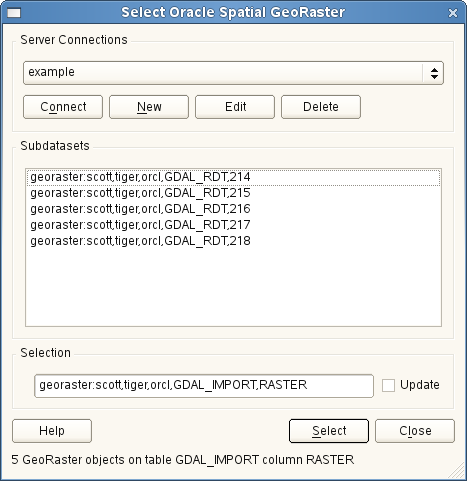
\includegraphics[clip=true, width=9cm]{oracle_select_dialog}
   \caption{Диалоговое окно <<Выберите Oracle Spatial GeoRaster>> \wincaption}\label{fig:oracle_select}
\end{figure}

Строка ввода блока <<Выделение>> также может использоваться для ввода
условия Where в конце идентификационной строки, к примеру
<<geor:scott/tiger@orcl,gdal\_import,raster,geoid=>>. Смотрите \\
\url{http://www.gdal.org/frmt_georaster.html} для более детальной
информации.

\subsection{Отображение растровых данных}

И напоследок, выбрав растровое изображение из списка таблица растровых
данных:идентификатор растрового изображения, в QGIS будет загружено
растровое изображение.

Теперь диалоговое окно <<Выбрать Oracle Spatial GeoRaster>> может быть
закрыто и в следующий раз при его вызове в нем будет отображаться то же
соединение, с тем же список подчиненных наборов данных, что облегчит
открытие другого изображения из того же окружения.

\textbf{Примечание:} растровые изображения, содержащие пирамиды, будут
отображаться быстрее, однако пирамиды должны быть созданы вне QGIS, с
применением Oracle PL/SQL или gdaladdo.

Вот пример использования gdaladdo:

\begin{verbatim}
gdaladdo georaster:scott/tiger@orcl,georaster\_table,georaster,georid=6 -r
nearest 2 4 6 8 16 32
\end{verbatim}

А это пример для PL/SQL:
cd ..
\begin{verbatim}
$ sqlplus scott/tiger
SQL> DECLARE
    gr sdo_georaster;
BEGIN
    SELECT image INTO gr FROM cities WHERE id = 1 FOR UPDATE;
    sdo_geor.generatePyramid(gr, 'rLevel=5, resampling=NN');
    UPDATE cities SET image = gr WHERE id = 1;
    COMMIT;
END;
/
\end{verbatim}

\FloatBarrier
